% Para facilitar a manutenção é sempre melhore criar um arquivo por capitulo, para exemplo isso não é necessário 

%---------------------------------------------------------------------------------------
\chapter{Etapas de Processo Seletivo}

O processo seletivo da Ernst & Young é dividido em seis etapas, as quais se estendem por um período de dez meses, sendo os dois primeiros meses apenas para inscrições, e, a partir do terceiro mês o processo avança para as etapas subsequentes, porém as inscrições permanecem até o último mês do processo.


\begin{figure}[h]
	\centering
	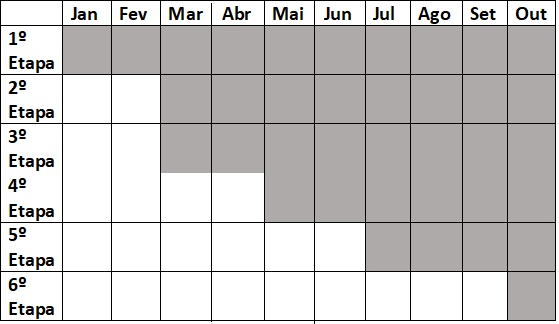
\includegraphics[scale=0.8]{processo.jpeg}
	\caption{Tempo total investido em cada etapa do processo seletivo}
	\label{fig:mesh1}
	
\end{figure}


\section{Inscrição e Avaliação Curricular}{

A avaliação curricular é uma etapa online que consiste em acessar o site do programa de \textit{Trainees} e realizar a inscrição, o que já direciona o candidato a vaga que mais adequada ao perfil do mesmo, e, além dessa maneira, as vagas ficas disponíveis em outras plataformas direcionadas ao recrutamento online, onde são amplamente divulgadas.
Na plataforma de recrutamento o processo seletivo fica mais acessível, pois, além de realizar cruzamento dos dados dos currículos como os pré-requisitos das vagas, onde sugere para os usuários vagas de acordo com o perfil do mesmo, também dá suporte durante o andamento de todas as etapas. 
Essa etapa garante uma maior agilidade e eficiência na análise de currículos de candidatos, além de tornar o processo mais visível por estar em uma plataforma na qual os usuários estão estritamente ligados para buscar uma vaga de emprego, onde a plataforma sugere para usuários a vaga com maior aderência.
As redes sociais também são amplamente utilizadas para divulgação do programa de \textit{Trainees} da EY, onde seus próprios colaboradores realizam postagens sobre o programa incentivando aos interessados a se inscreverem na oportunidade.
Nessa etapa os candidatos são analisados e selecionados com base nos requisitos mínimos preestabelecidos com base em sua formação e habilidades específicas (neste caso o Inglês).


\begin{table}[htb]
\centering
\caption{Pré-requisitos}
\label{tab-exemplo}
\begin{tabular}{p{2.8cm}|r|r|r|r}
    \hline
   \textbf{Curso} & \textbf{Formação}  & \textbf{Nível de Inglês} \\
    \hline
    Ciências Contábeis & Janeiro de 2017 a dezembro de 2022 & Básico  \\
    \hline
    Cursos de T.I. & Janeiro de 2017 a dezembro de 2021  & Básico \\
    \hline
    Administração de Empresas, Ciências Atuariais, Economia, Relações Internacionais, Comércio Exterior, Direito, Engenharia (todas), Estatística, Física, Matemática, Psicologia, Marketing, Publicidade e Propaganda, Design & Janeiro de 2017 a dezembro de 2021  & Intermediário \\
    \hline
\end{tabular}
\fonte{Disponível em: <https://beyellow.com.br/programa/>. Acessado em: 23 de Setembro de 2020}
\end{table}}



\newpage


\section{Apresentação Institucional e Redação}

A etapa de apresentação é presencial, realizada na Universidade Corporativa da EY, onde cerca de 50 candidatos que foram classificados na etapa dos testes online, são direcionados para uma palestra de apresentação da empresa, suas diversas áreas com vagas disponíveis, o programa de \textit{Trainees} e seus benefícios. Os candidatos ainda podem tirar dúvidas sobre o processo seletivo e a empresa.
Após a apresentação, o candidato recebe uma folha para fazer uma redação, referente a um tema específico, ligado diretamente à proposta e visão da empresa, que é fazer um mundo de negócios melhor. Com quantidade mínima e máxima de palavras, com um intervalo de tempo de 1 hora. 
Essa etapa da ao candidato a possibilidade de especificar a área da empresa na qual deseja atuar, podendo escolher uma ordem de prioridade entre 3 áreas. Sendo assim, o candidato aprovado será direcionado entre as vagas das áreas priorizadas por ele.
Nessa etapa é analisada a capacidade de comunicação escrita dos candidatos, além da capacidade da abordagem correta do tema e a área de atuação escolhida, em relação as vagas disponíveis.




\section{Testes Online e Escolha da Área de Interesse}

Após a avaliação dos pré-requisitos, a redação e escolha da área de atuação, essa etapa consiste em testes online de Português, Lógica, Inglês em caráter eliminatório e Contabilidade Básica em caráter classificatório, esse último sendo apenas para os cursos de Ciências Contábeis, Administração de Empresas e Ciências Atuariais.
Essa etapa consiste em teste de múltipla escolha, com questões que evoluem de básicas a avançadas de cada assunto, para que o candidato seja avaliado e de acordo com a pontuação, mínima de 70\% em cada teste.
Durante essa etapa são avaliados de maneira eliminatória e classificatória conhecimentos gerais necessários, como Português, Lógica e Inglês, e específicos, no caso de Contabilidade Básica.



\newpage

\section{Dinâmica de Grupo}

A etapa de dinâmica de grupo é presencial com 10 candidatos que, inicialmente, são submetidos a um teste, onde devem desenhar uma casa, árvore e uma pessoa, conhecido como teste de personalidade HTP.
Esse teste tem como objetivo mostrar quais são os conflitos escondidos e comuns dentro de cada candidato, além disso o entrevistador pede para que os candidatos se apresentem e solicita que respondam algumas perguntas como: porque quer trabalhar na EY, o que espera do processo, qual é a maior área de interesse de atuação de acordo com o curso, além de explicar o porquê desenhou os elementos solicitados como desenhou.
Após a primeira fase das dinâmicas os candidatos são divididos em dois grupos com cinco participantes cada, onde é apresentado aos grupos um \textit{case} relacionado com a área de atuação na qual os candidatos foram selecionados. Vale evidenciar, que os grupos são mistos, incluindo candidatos dos vários ramos das vagas disponíveis.
Com isso, o grupo tem um tempo limite de dez minutos para desenvolver o \textit{case}, e organizar uma apresentação, com apoio de uma cartolina, com o desenho da solução e desenvolver um \textit{pitch} de três a cinco minutos,onde os grupos são concorrentes e ambos devem tentar convencer o entrevistador a comprar sua solução proposta. Nessa fase da dinâmica, os candidatos serão pressionados pelo entrevistador durante a apresentação, visando colocá-los em um cenário de extrema pressão e desconforto, e, após a conclusão da apresentação, o outro grupo também pode realizar perguntas.
Após o término das apresentações, o entrevistador dá um \textit{feedback} para os grupos, dizendo os pontos fracos e fortes desenvolvidos durante o \textit{case} e expõe que o objetivo da etapa é uma experimentação para saber como cada candidato se sai sob pressão.
Ao final, abre para perguntas e dúvidas relacionadas a empresa e ao processo seletivo.
Durante essa etapa são avaliador quesitos de personalidade dos candidatos, capacidade de desenvolver uma história, liderança, capacidade de trabalho em equipe, capacidade de trabalho sob pressão, capacidade de comunicação verbal e visão ampla de negócios.




\section{Entrevistas Finais}
Essa etapa é subdividida em duas entrevistas de cerca de 30 minutos cada, onde é realizada uma conversa entre o candidato e o Gerente Técnico, e o candidato e um Sócio da EY.


Durante a entrevista com o gerente são feitas perguntas referentes a formação, áreas de interesse e áreas de atuação. Ainda é feito um \textit{case}, onde é avaliada a tomada de decisão do candidato.
Ao final, a entrevista se abre para perguntas, estipulando um limite máximo de perguntas, onde são avaliadas as perguntas feitas pelo candidato, visto que se espera perguntas que consigam extrair boas informações referente aos negócios e carreira.
Durante a primeira entrevista são avaliados conhecimentos técnicos, tomada de decisão, formulação de perguntas e extração de informações.
    
Durante a entrevista com o sócio são feitas algumas perguntas referentes aos objetivos profissionais e áreas de atuação. Novamente é feito um \textit{case}, onde é dada uma situação hipotética ao candidato e é solicitada uma solução objetiva para o caso, com tempo de cinco minutos. Além disso, é dado papel e caneta para que o candidato possa rascunhar sua solução, visto que envolve cálculos. Após dar a solução, é necessário explicar o raciocínio seguido.
Ao final, a entrevista se abre para perguntas, estipulando um limite máximo de perguntas, novamente avaliando as perguntas feitas pelo candidato.
Durante a segunda entrevista são avaliadas a linha de raciocínio do candidato, capacidade de formulação de perguntas e extração de informações.

Ao final, os dois, juntamente com o entrevistador da dinâmica em grupo, fazem uma reunião, onde classificam todos os candidatos entrevistados, definindo os pontos fortes e fracos dos candidatos, além de definir qual será a área inicial de cada candidato.
Vale ressaltar, que essa entrevista é dinâmica, visto que cada entrevistador e cada candidato tem perfil próprio, o ponto em comum entre todas são os pontos de avaliação que os entrevistadores devem extrair com a conversa.


\section{Processo Admissional}
Ao fim de todos os processos a empresa entra em contato com os candidatos, dando o \textit{feedback} positivo ou negativo e informando o motivo dos mesmos. Em casos positivos, é feita a proposta para o candidato. Após a aceitação, o mesmo é instruído a enviar os dados para admissão, e, posteriormente, para realizar o exame admissional. Depois disso, o novo colaborador é apresentado aos termos do contrato, assina a documentação e inicia sua atuação na empresa.